%!TEX root = ../paper.tex
%Concept is more general where as implementation is solving problems with the specific domain/data
\section{Concept}
\label{sec:concept}
We now present our approach to the \nto problem.
The next section details our two-staged classification approach.
We then talk about what features we select and how we approach the \todo{\emph{documentmismatch}}.

\subsection{Two-staged classification}
As presented in Section~\ref{sec:background-problem} there exist the problem, that brochures are not written from the user perspective.
We called this the \emph{non-user perspective problem}.
In fact, there also exist two concepts in the posts.
These concepts are orthogonal to each other and are shown below.

First, users might express a need, demand, or interest for some product or not.
This might be a product of our company or not.
Typical phrases, taken from an experiment on our example data set (see Section~\ref{sec:evaluation}), for this concept are:
\begin{center}
	\textit{need, hi, looking for, recommend, please, anyone, appreciate, thank you}
\end{center}
We call this the \emph{demand classification}:
\begin{align*}
	\mathbf{demand}&: POSTS \longrightarrow \big\{ \operatorname{``demand''}, \operatorname{``no-demand''} \big\}
\end{align*}

The second concept is about which product the user is talking about in the post.
Here, the decision needs to be made whether this is a product of the company or not.
In the latter case, we are not interested in the post anymore.
Depending on the actual product, the relevant words vary greatly.
The following words are relevant words for a customer relationship managment software, also taken from our example data:
\begin{center}
	\textit{customer, sales, crm, b2b, consumer, salesforce, organization, account}
\end{center}

We call this the \emph{product classification}:
\begin{align*}
	\mathbf{product}&: POST \longrightarrow  PRODUCT \cup \big\{ NONE \big\}
\end{align*}

The intersection of the most relevant words for demand and product classification is the empty set.
This observation shows, that these concepts are independent of each other and should be treated separately.
If a post is about a product of the company, that does not necessarily mean, that the system should make a recommendation and vice versa.
Demand posts and posts about one of ACME's product have different characteristica, which should be represented in the system's architecture.

Therefore, we split the \nto problem in two subproblems: given a post $p \in POSTS$ we first identify, whether the posts expresses a demand for any product in general.
If this is true, we then check whether we can actually categorize the post into one of ACME's products.
All together, given $demand$ and $product$, we can define \nto:

\todo{Reference it!}
\begin{equationBlock}
	\label{equation:two-stages}
	\begin{alignat*}{3}
	  &\mathbf{NTO}: && ~POSTS && \longrightarrow PRODUCT \cup \big\{ NONE \big\} \\
	  &\mathbf{NTO}: && ~~p   && \longmapsto \begin{cases}
		    product(post)~~~~~~~\text{if }~demand(post) = \operatorname{``demand''} \\
		    NONE~~~~~~~~~~~~~~~\text{otherwise}
	   \end{cases}
	\end{alignat*}
	\caption{Defining \nto via two-staged classification.}
\end{equationBlock}

In our system, both $demand$ and $product$ are implemented by two independent text classification algorithms.
We are using supervised machine learning for this.
Supervised learning requires tagged training samples to draw conclusions on unseen test samples.

The training data for the $demand$ classifier comes from posts from social media networks.
This requires manually classifying posts into ``demand'' and ``no-demand''.
We did this manually for a sample of social network posts.
However, the demand classification does not change for different companies or products.
It is independent from the product classification, which is why companies do not need to supply training data for the demand classification.
Rather, they can use a prebuilt demand classifier.

The training data for the $product$ classifier needs to be supplied in form of brochures and/or marketing material for the different products.
Each brochure must be assigned to one product.
There can be more than one product.
The system then automatically learns from the brochures.
Figure~\ref{fig:workflow} illustrates the architecture of the system. \todo{How does Figure\ref{fig:figureone} differentiate from Figure\ref{fig:workflow}. We should not show the sames figures twice}

\begin{figure}
	\label{fig:workflow}
	\begin{center}
		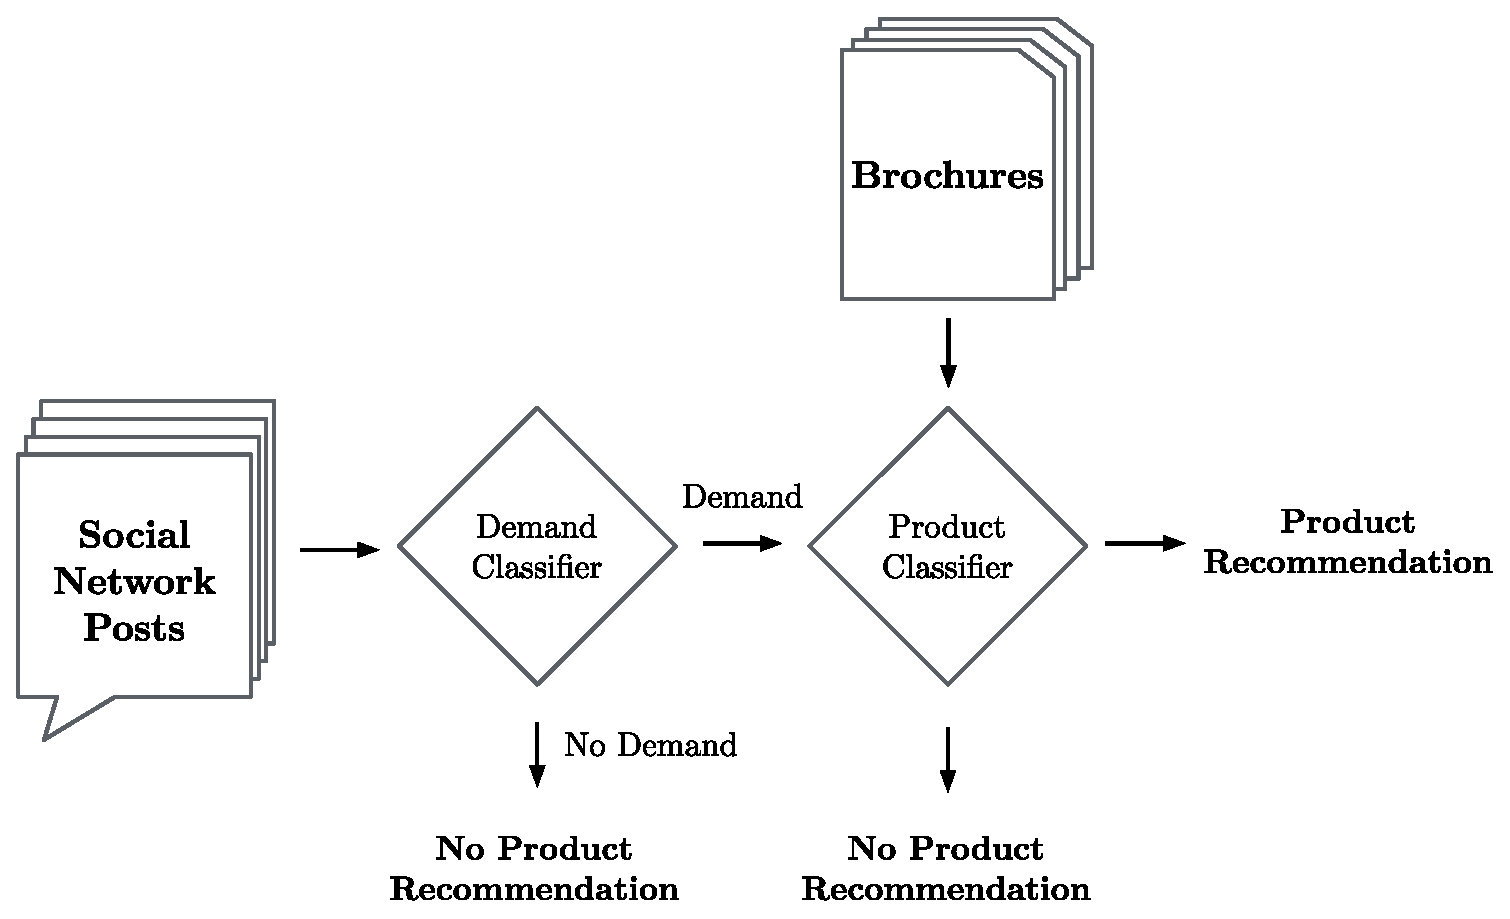
\includegraphics[width=0.7\textwidth]{figures/nto_workflow.eps}
	\end{center}
	\caption{Together, a demand classifier training from social network posts and a product classifier trained from marketing material form a classification-model for unseen posts.}
\end{figure}

Learning demand and product categorization as two concepts with different classifiers also helps overcome data sparsity issues.
The number of posts that actually are asking for a product of the company is usually very low.
In our example data set, these posts only cover \todo{XX}~\% of the posts, whereas demand posts occur with \todo{XX}~\% probability and product documents with \todo{XX}~\%.
If the machine learning would work directly on the positive examples, this would introduce a high data skew.
The number of positive training samples would be at least a magnitude lower than the number of negative samples.
This skew has been shown to harm the performance of machine learning systems significantly \cite{monard2002learning,guo2008class}.

However, even with two classifiers, the number of positive samples is much lower than the number of negative examples.
Therefore, we employ techniques of feature selection and training data sampling, which are shown in the next two sections.

\subsection{Feature Selection}
\label{sec:feature-selection}
As we use supervised machine-learning for the text categorization, we need to define features, which are good for predicting a demand and a certain product.
The general approach to features in text classification is the bag-of-words model \cite{yang1997comparative,zhang2010understanding}.
This model treats each text as a multiset of words in the text.
This approach loses the text order, but keeps the information about the frequency of words.
Our classifiers are based on a bag-of-word approach.

Because we have both the \emph{problem of document mismatch} and the \emph{problem of a small corpus}, we use a strict feature selection to avoid any overfitting to the training data and selecting the wrong words.

For the demand classifier, the first observation is, that there no specific words for no-demand posts.
Almost every randomly selected post does not express a demand, and it could be about any topic.
Therefore, we choose to select only words, which express a demand (e.g. ``recommend'', ``help'', ``looking'', ``need'').
The intuition is, that if enough of demand words occur, we classify a demand, otherwise a no-demand.
To identify these words we run two statistics on the data:
which words are more likely to occur in demand-posts, and which words are more likely to not occur in no-demand posts.
\begin{figure}
	\label{eq:demand_feature_selection}
	\begin{alignat*}{3}
		&demand\_prob\_with(w) &&= \dfrac{
		 		\#~\operatorname{demand}~posts~\mathbf{with}~w
			}{
				 \#~\operatorname{demand}~posts
			}
			\\
		&no\_demand\_prob\_with(w) &&= \dfrac{
		 		\#~\operatorname{no-demand}~posts~\mathbf{with}~w
			}{
				 \#~\operatorname{no-demand}~posts
			}
			\\
		&demand\_fraction\_with(w) &&= \frac{
				demand\_prob\_with(w)
			}{
				no\_demand\_prob\_with(w)
			}
			\\[2mm]
			\hline
			\\[0.1mm]
		&demand\_prob\_without(w) &&= \dfrac{
		 		\#~\operatorname{demand}~posts~\mathbf{without}~w
			}{
				 \#~\operatorname{demand}~posts
			}
			\\
		&no\_demand\_prob\_without(w) &&= \dfrac{
		 		\#~\operatorname{no-demand}~posts~\mathbf{without}~w
			}{
				 \#~\operatorname{no-demand}~posts
			}
			\\
		&demand\_fraction\_without(w) &&= \frac{
				no\_demand\_prob\_without(w)
			}{
				demand\_prob\_without(w)
			}
	\end{alignat*}
	\caption{The demand feature selection is based on the two functions $demand\_fraction\_with$ and $demand\_fraction\_without$, which select words, that are an indication for a demand post.}
\end{figure}
We select those words with the highest $demand\_fraction\_with$ and the highest $demand\_fraction\_without$.
The final demand words is the set union of these two sets.
These words indicate a demand: if they do occur, then that is a sign for a demand post, if they do not occur, then that is a sign for a no-demand post.
Using this approach we can overcome the \emph{small corpus problem} for the demand posts.

For the product classifier we use a classical tf-idf\cite{sparck1972statistical} feature selection.
Often, only a few keywords indicate membership to a product class.
Tf-idf helps to find these words, while ignoring words that may occur in every brochure, like the company name, stop words or generic words.
% The demand classifier is trained on social network posts and also predicts on social network posts.

% document mismatch --> strict feature selection
% small corpus --> training data generation

\subsection{Training data generation}

As said before, the number of brochures is usually quite low, hence there is not much training data.
Also, there exists a mismatch between the posts and the brochures.
One part of this document mismatch is, that brochures are usually much longer than social network posts, which often only contain two or three sentences, while brochures span over pages.
Hence, a natural approach is to split one long brochure into several smaller brochures, which both creates more training data and adapts the document length closer to the post's document length.
